\newif\ifvimbug
\vimbugfalse

\ifvimbug
\begin{document}
\fi

\exercise{Expectation Maximization}
 
In this exercise, you will use the datasets \texttt{gmm.txt}. It contains data from a Gaussian Mixture Model with four 2-dimensional Gaussian distributions.

\begin{questions}

%----------------------------------------------

\begin{question}{Gaussian Mixture Update Rules}{2}
Define the model parameters and the update rules for your model. 
Specify the E- and M-steps of the algorithm.

\begin{answer}\end{answer}

\end{question}

%----------------------------------------------

\begin{question}{EM}{18}
Implement the Expectation Maximization algorithm for Gaussian Mixture Models. Initialize your model uniformly. Generate plots at different iterations $t_i \in [1,3,5,10,30]$, showing the data and the mixture components, and plot the log-likelihood for every iteration $t_i=1:30$. Attach a snippet of your code.
\begin{figure}[]
	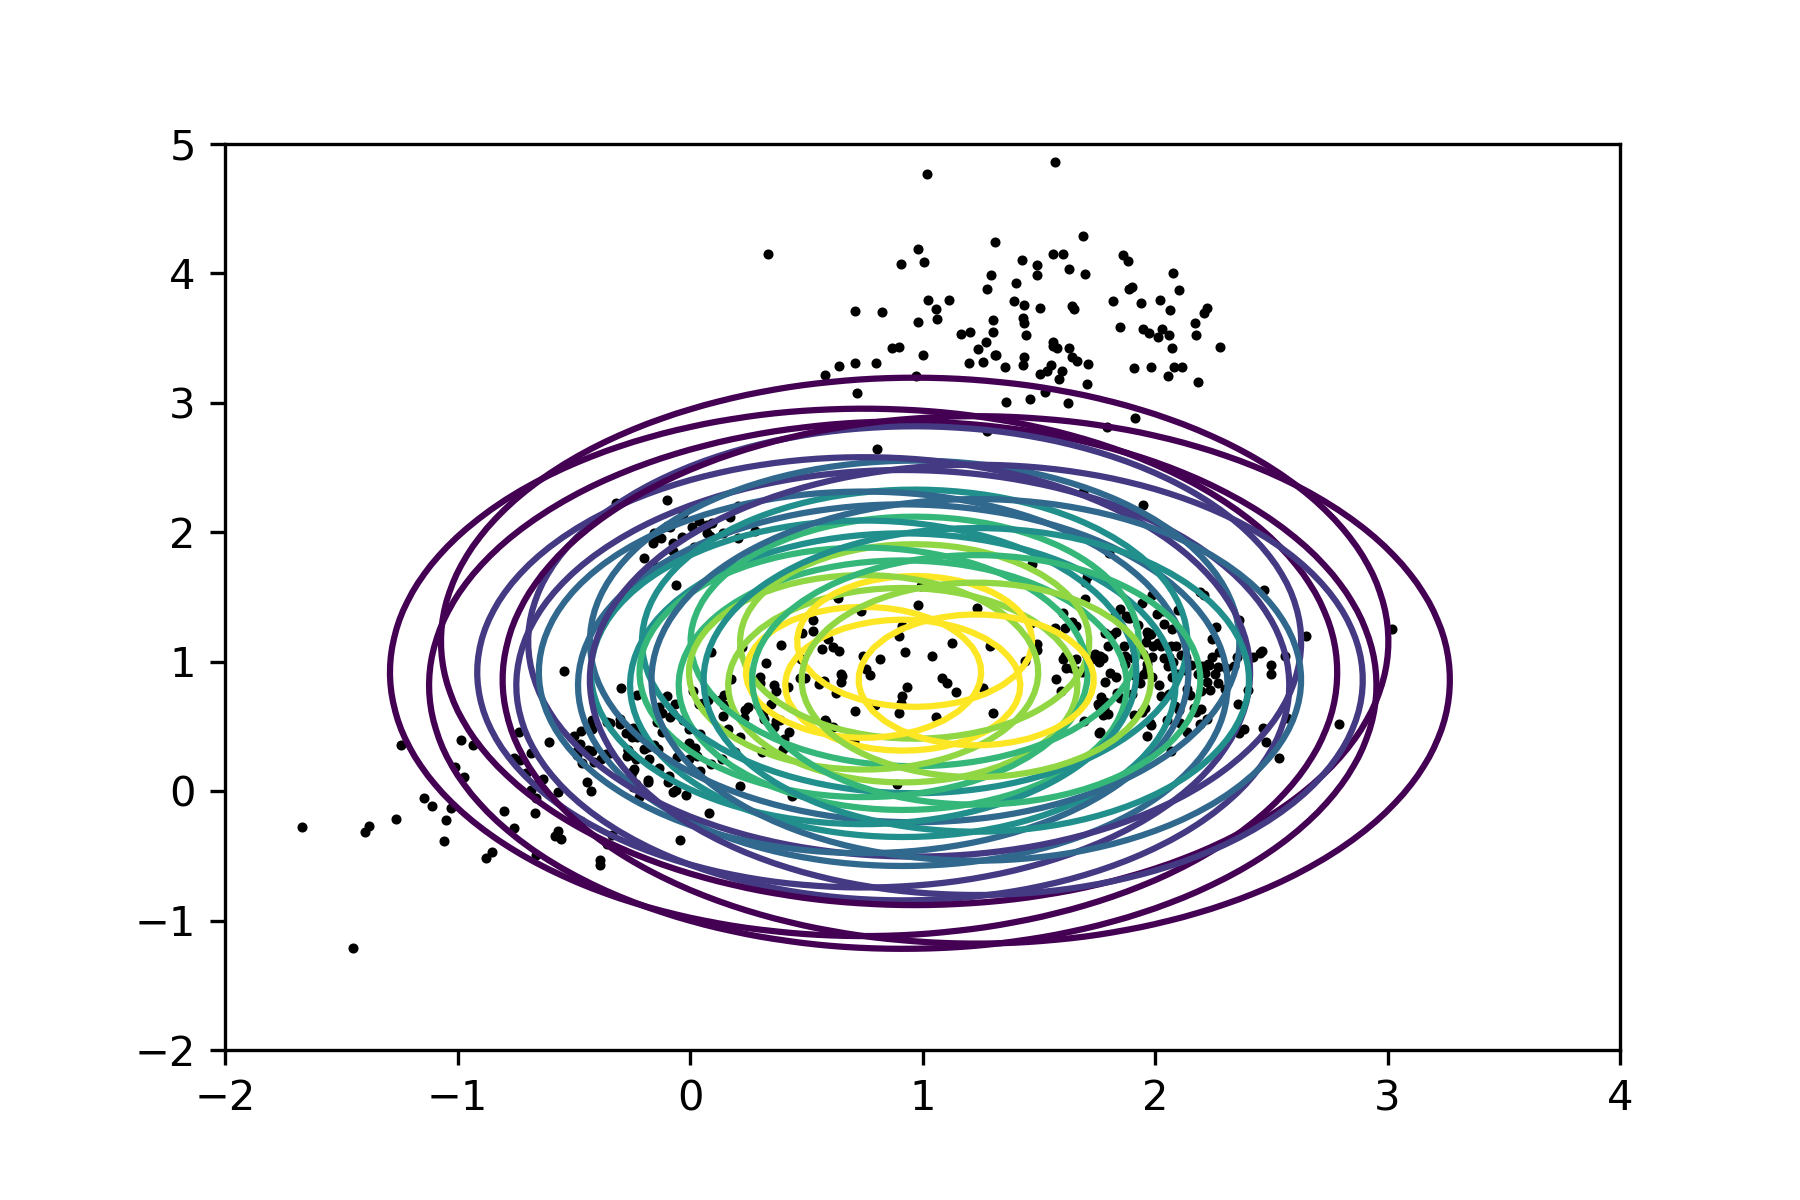
\includegraphics[width=0.8\linewidth]{pictures/em_iter_1.png}
	\centering
	\caption{Plot of mixture components and data after 1 iteration.}
	\label{fig:1}
\end{figure}
\begin{figure}[]
	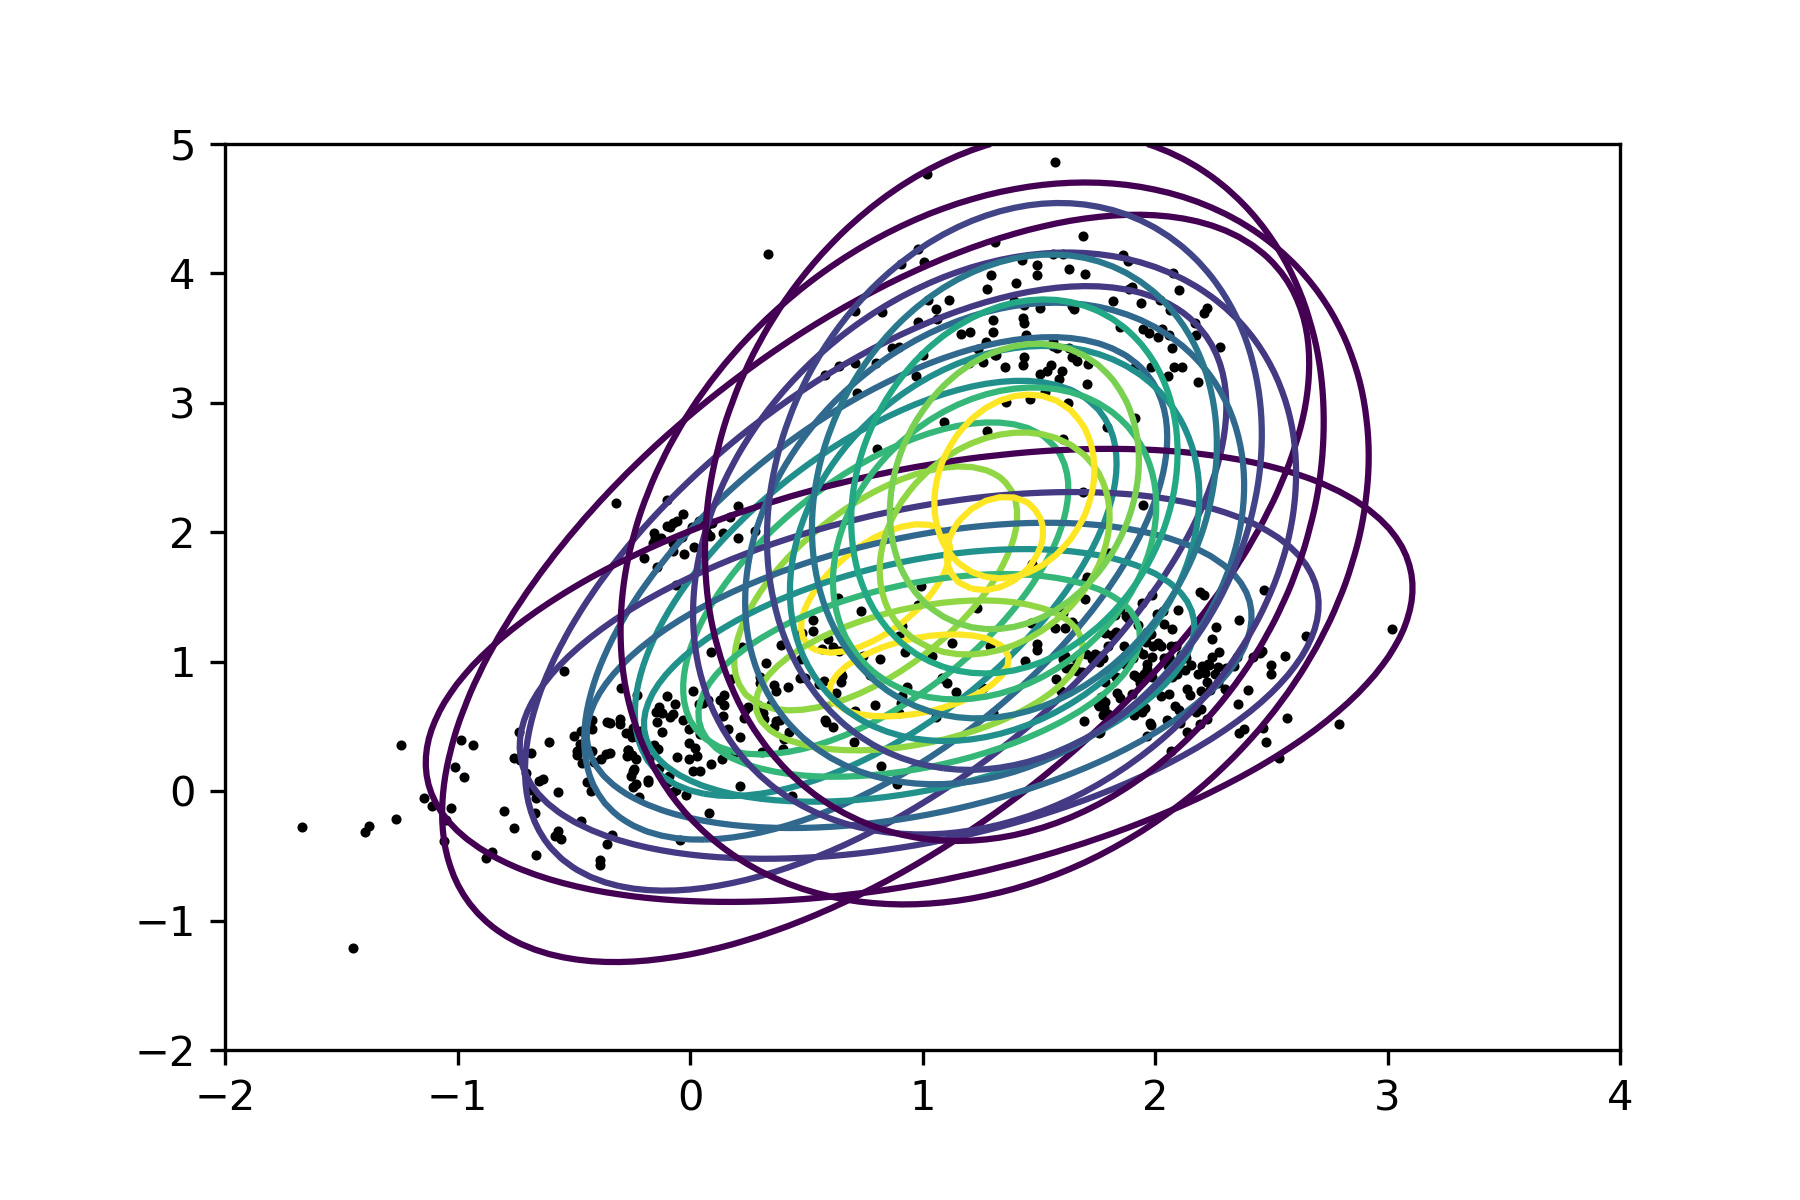
\includegraphics[width=0.8\linewidth]{pictures/em_iter_3.png}
	\centering
	\caption{Plot of mixture components and data after 3 iterations.}
	\label{fig:2}
\end{figure}
\begin{figure}[]
	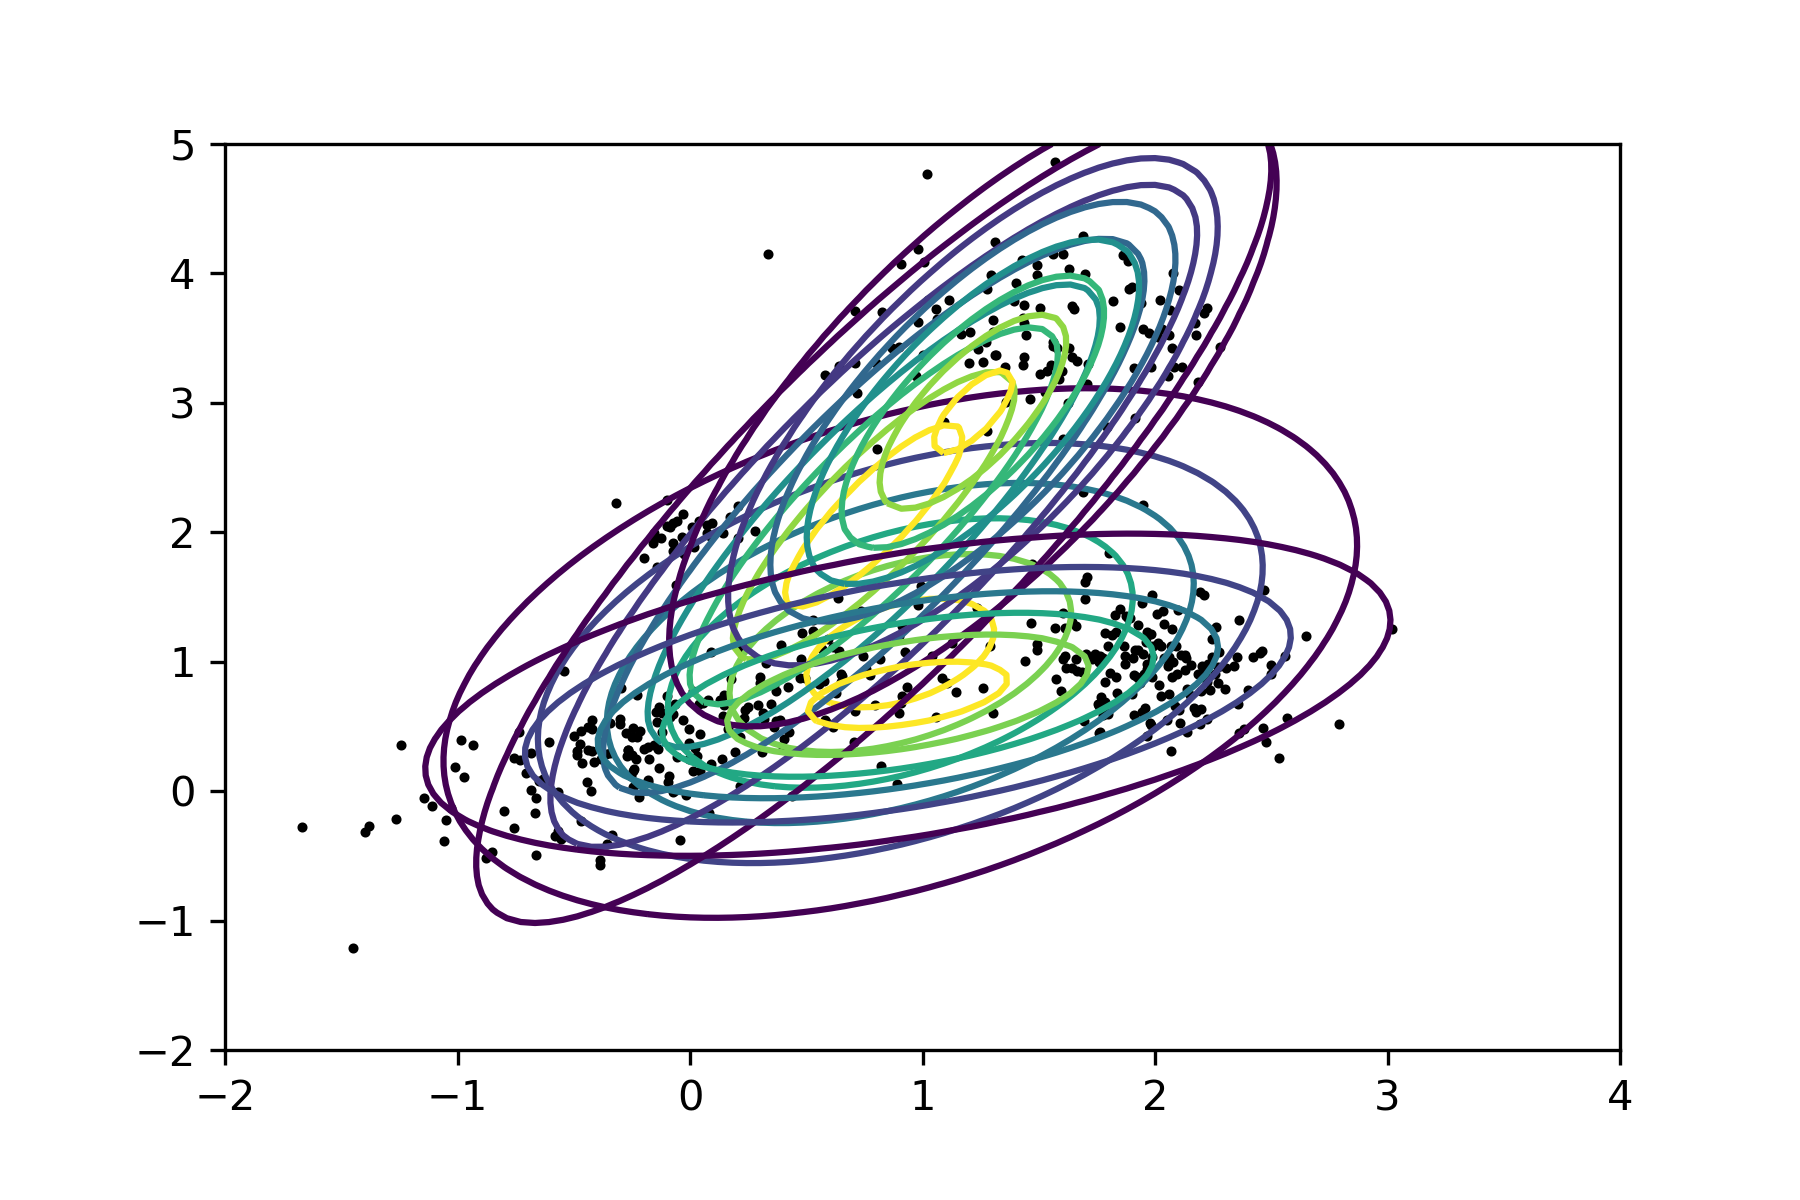
\includegraphics[width=0.8\linewidth]{pictures/em_iter_5.png}
	\centering
	\caption{Plot of mixture components and data after 5 iterations.}
	\label{fig:5}
\end{figure}
\begin{figure}[]
	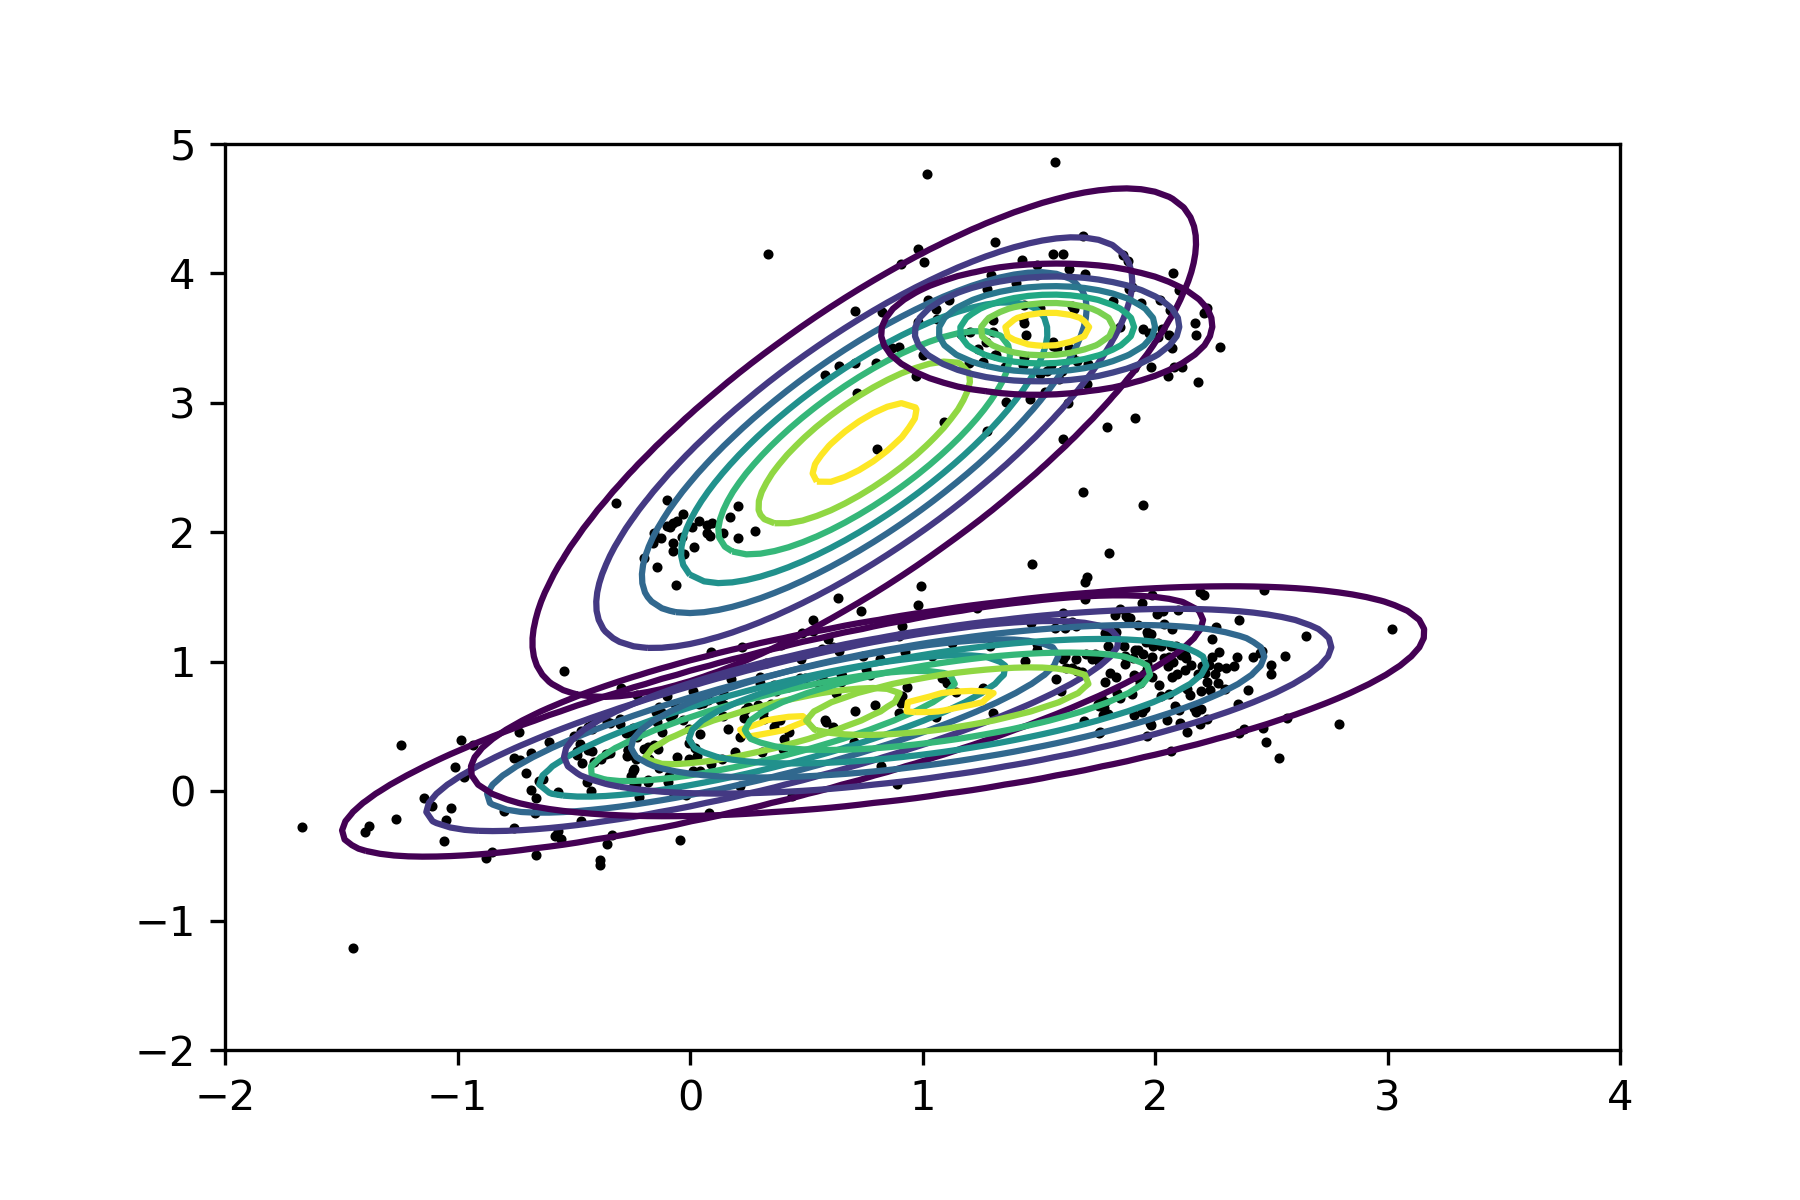
\includegraphics[width=0.8\linewidth]{pictures/em_iter_10.png}
	\centering
	\caption{Plot of mixture components and data after 10 iterations.}
	\label{fig:10}
\end{figure}
\begin{figure}[]
	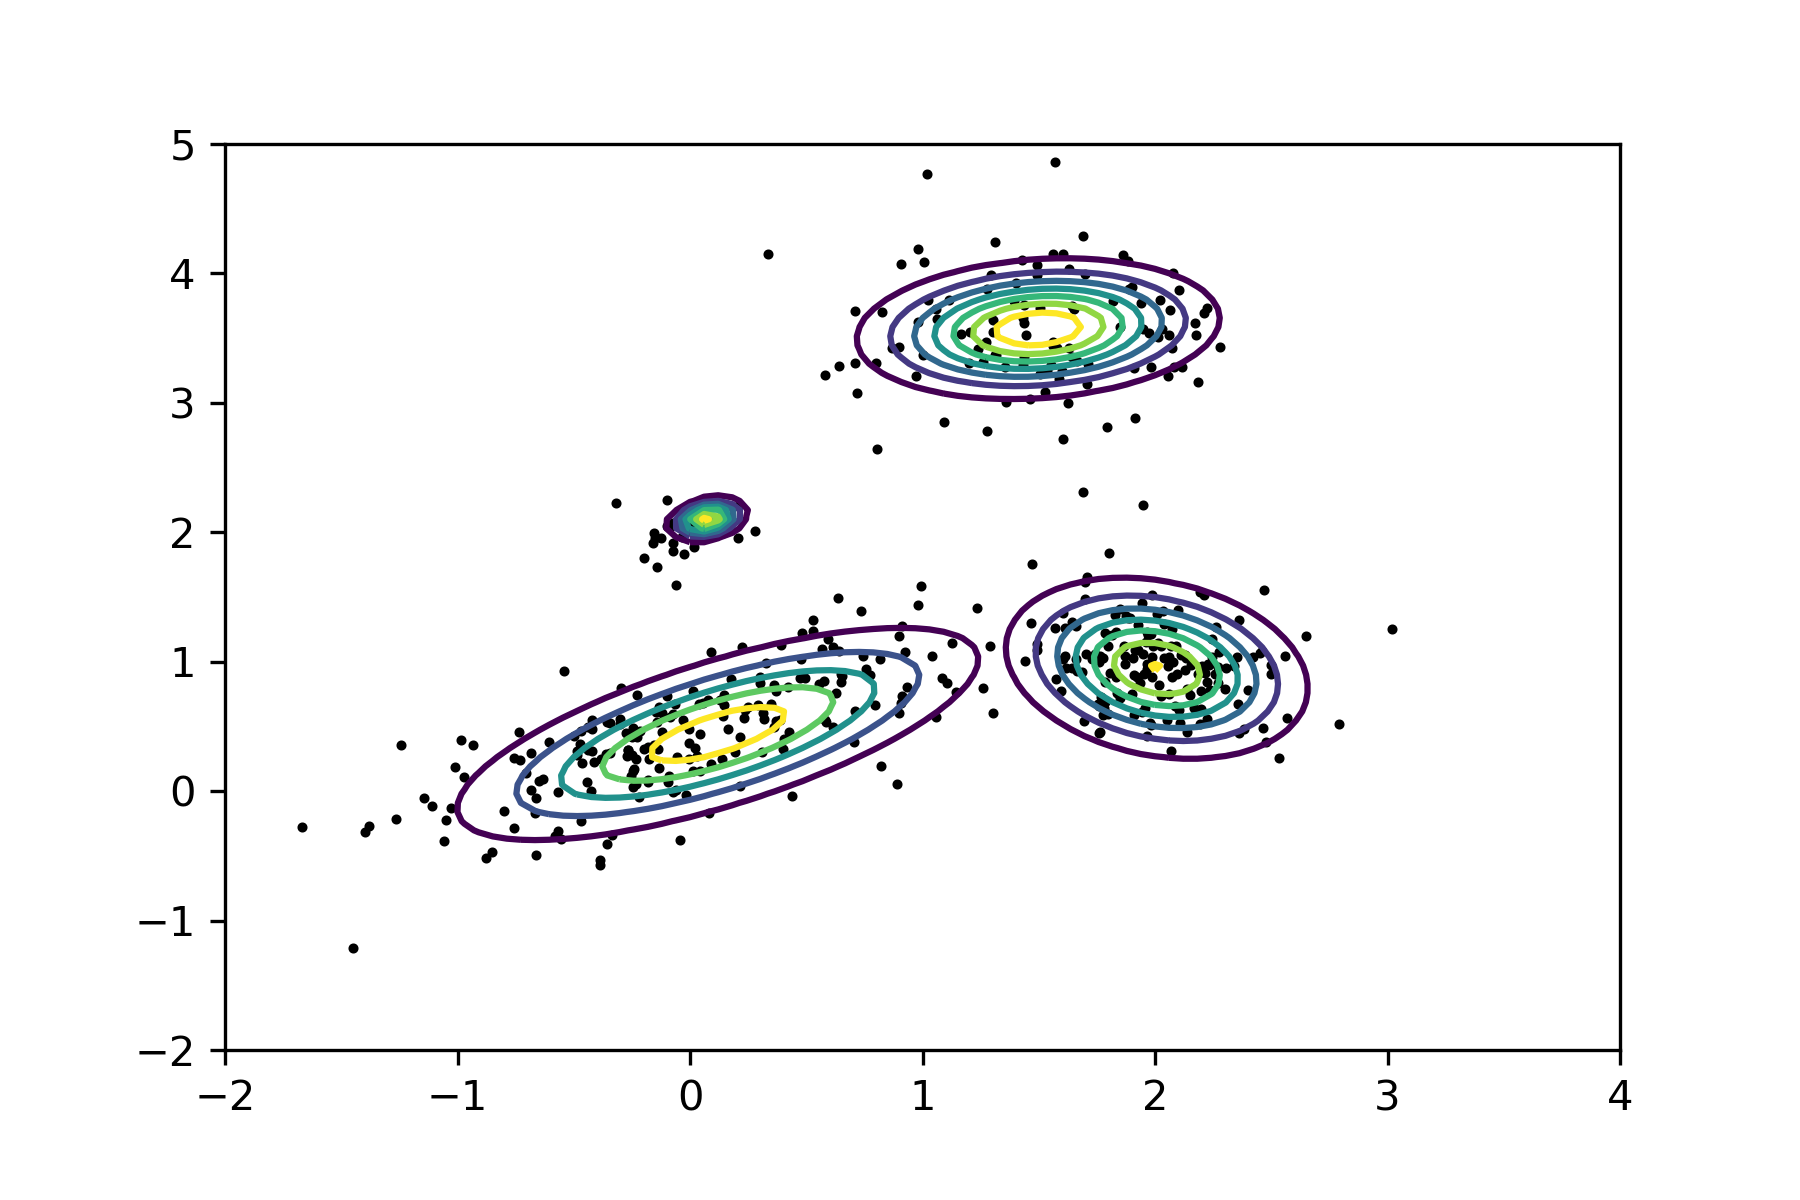
\includegraphics[width=0.8\linewidth]{pictures/em_iter_30.png}
	\centering
	\caption{Plot of mixture components and data after 30 iterations.}
	\label{fig:30}
\end{figure}
\begin{answer}
For the iterations $t_i \in [1,3,5,10,30]$we obtain the following plots with the data and the mixture components.\\
The code of the EM implementation is attached:
\lstinputlisting[language=Python]{EM_hw.py}
\end{answer}

\end{question}

\end{questions}
